\documentclass[12pt]{article}
\usepackage{amsmath}
\usepackage{hyperref}
\usepackage{color}
\usepackage{amsthm}
\usepackage{graphicx}

\title{Project Proposal} 
\author{Sean Smith, Viviana Yee \\ \{swsmith, vivyee\}@bu.edu}
\date{15 March 2017}

\begin{document}
\maketitle


\section{Problem Definition}
	The city of Boston maintains an open data initiative that provides datasets on lots of different city services \url{https://data.cityofboston.gov/}. We both have experience taking large amounts of data and making conclusions based on trends and correlations between different datasets. Based on Viviana's experience in Andrei Lapet's Data Mechanics Course and Sean's experience with New York City Taxi data and geographical zone information we've decided to look at Boston obesity data and locations of nutrition centers and the distance between them. Specifically we want to model MBTA transportation options from different neighborhoods (for which we're able to calculate the obesity rate) to nutrition centers. We aim to model the distance in order to answer our hypothesis "Do neighborhoods further from nutrition centers suffer from greater obesity rates?". 
 
 \section{Data Sources}
	First we needed to define the geographic areas that we'll be modeling, to do so we've downloaded the 2010 census tracts dataset. This breaks Boston up into unique tracts that each have approximately the same number of residents. You can see an example below:

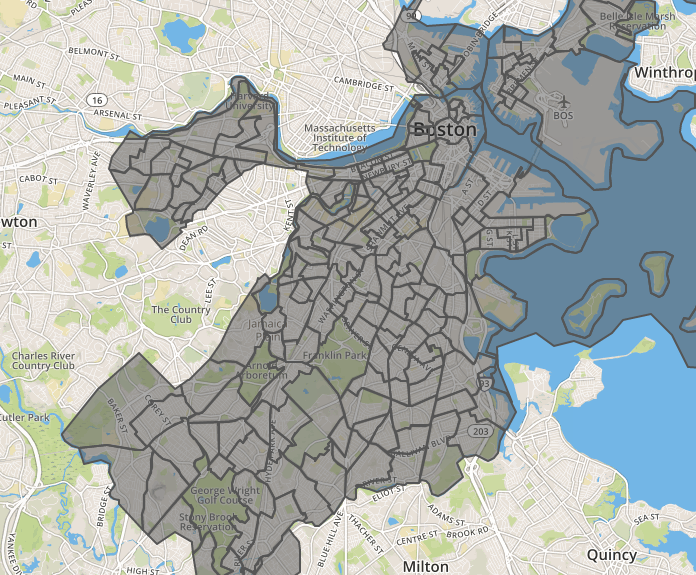
\includegraphics[height=4in]{boston_neighborhoods.png}

Next, we took Obesity data from the CDC, Center for Disease Control, and Nutrition Program data from the city of Boston. We filtered these two data sets for longitude and latitude data, so it is valuable for our problem.

Finally, we called the MBTA API endpoints for MBTA stop data. We did this by getting routes for the bus and T. From that, we individually got all stops for each route because there is no API call for all stops in the MBTA system. 

 By modeling our data with propositional logic we hope to answer the following questions. 
 
 \begin{itemize}
 \item Do neighborhoods further from nutrition centers suffer from greater obesity rates?
 \item Do neighborhoods with more than one nutrition center have lower rates of obesity?
 \item Does the obesity rate in surrounding neighborhoods change your neighborhood's access to nutrition centers?
 \end{itemize}

 \section{Methodology}

We're getting datasets from Boston Open Data portal using python and their API's. We're then solving for satisfiability of our WFF's using Z3 \url{https://github.com/Z3Prover/z3}.

We're doing the following experiments:

\begin{enumerate}
\item We're solving for the satisfiability that a coordinate pair is contained in a certain neighborhood. This uses the point in polygon algorithm that Sean developed for the Multi Party Computation class.
\item Find shortest path to all nutrition programs and find shortest out of that
\item Pick a neighborhood with a nutrition program that is geographically closest, and find shortest path to that
\item Combine (find all neighborhoods within certain distance and calculate shortest path for programs within the radius)
\item Find shortest path from every neighborhood to every nutrition center (depends on running time)
\end{enumerate}


\end{document}